\documentclass[../main.tex]{subfiles}

\begin{document}
\chapter{The Website — Designing and Implementing an Elegant Interface} \label{ch:website}
    There were two options for how to implement the user interface: a desktop
        application or a website.
    A desktop application would have allowed users to run their programs locally,
        safely using any Haskell library they wanted.
    However, this would have required users to install the application, and Haskell
        itself, which could alienate users who are unfamiliar with installing software.
    A website would allow users to run their programs in the browser, without need
        to install anything.
    This would make the system more accessible to users, and compatible across
        multiple platforms.
    For these reasons, the system was implemented as a website.

    The website is the interface for users to interact with the system, so it was
        important that the website be user-friendly and easy to use.
    This chapter discusses its design, implementation, and the technologies used to
        build it.

    \section{Design Principles}
        Websites have been at the core of people's lives for the past two decades.
        They are used for a variety of activities, from shopping to socialising to
            filing taxes.
        It is thus essential that websites meet certain design standards, to ensure
            that users can easily navigate and interact with them.
        It is also important that websites are visually appealing, to keep users
            engaged.
        Due to these requirements, many standard design practices have emerged, which
            are important to consider when designing a website.

        \subsection{Purpose — What is the site for and how do we achieve that?}
            The first thing to consider when designing a website is its purpose.
            For this project, the website was designed to allow users to write and run
                programs in Haskell.
            It had to integrate seamlessly with the graphics library discussed in
                Chapter~\ref{ch:graphics}, and render both the textual and graphical results of
                programs.

            It would have been easy to say that an editor for Haskell, integrated with the
                graphics library, and a way to execute programs would be sufficient, and to
                ignore any further functionality.
            However, this would have been a mistake.
            The website had to be designed with user-friendliness in mind, and to provide
                users with all the tools and information they might need.
            This meant that the website would need four main pages:
            \begin{itemize}
                \item The editor, integrated with the graphics library, for users write, run, save
                      and share their programs.
                \item The reference page, for users to learn how to use the graphics library.
                \item The homepage, to showcase the capabilities of the library and encourage
                      users to try it out.
                \item The account page, for users to view and manage their saved programs and their
                      account settings.
            \end{itemize}
            There were a few additional pages, such as a login page, a registration page,
                and a privacy policy page.

        \subsection{Key Considerations}
            \subsubsection{User Experience — How can we make the website easy to use?}
                A website should be easy to use, with a clear and intuitive interface that
                    guides users through the various features and functions of the site.
                Most websites follow a standard layout (see Figure~\ref{fig:webLayout}), with a
                    header at the top of the page containing the site's logo and navigation links,
                    a main content area in the centre of the page, and a footer at the bottom of
                    the page for additional links and information.
                It is also recommended limiting text to between 45 and 75 characters wide, as
                    longer or shorter lines make it difficult for users to read \citep{lineLength}.

                \begin{figure}[H]
                    \centering
                    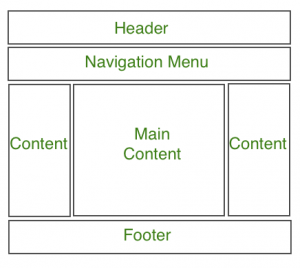
\includegraphics[width=0.35\linewidth]{images/webLayout.png}
                        \caption{Standard website layout.
                            Image taken from \href{https://www.geeksforgeeks.org/css-website-layout/}{Geek
                                    for Geeks: CSS Website Layout}.
                        }
                        \label{fig:webLayout}
                \end{figure}

            \subsubsection{Visual Design — How can we make the website visually appealing?}
                The website should be visually appealing, with a clean and modern design to
                    reflect the brand and purpose of the site.
                It should use a consistent colour scheme, and typography with clear and legible
                    text.
                Images and graphics can enhance the visual appeal of the site, but should be
                    used sparingly and to complement the overall design \citep{images}.
                For this site, it made sense to use a colour scheme based on the Haskell logo
                    (see Figure~\ref{fig:haskell}) to reflect the use of Haskell.

                \begin{figure}[H]
                    \centering
                    
\includegraphics[width=0.2\linewidth]{images/haskell.png}
                    
\includegraphics[width=0.2\linewidth]{images/haskellGrey.png}
                        \caption{Coloured Haskell logo (left) and monochrome Haskell logo (right).
                            Images taken from \href{https://www.haskell.org/}{Haskell.org} and
                                \href{https://wiki.haskell.org/Haskell_logos}{Haskell Wiki}.
                        }
                        \label{fig:haskell}
                \end{figure}

            \subsubsection{Accessibility — How can we make the website accessible to all users?}
                Accessibility is essential, and often overlooked, when designing a website.
                Websites should be accessible to all users, including those with disabilities,
                    or visual impairments such as colour blindness.
                To keep accessibility in mind, basic features such as alt text for images, high
                    contrast text, and semantic HTML for screen readers should be used.
                Websites should also be responsive, adapting to different screen sizes and
                    devices.

    \section{Technologies}
        There were a number of technologies used to implement the website.
        While all websites are built with some combination of HTML, CSS, and
            JavaScript, there are a number of frameworks, libraries and tools to make the
            development process easier and more efficient.

        \paragraph*{TypeScript}
            TypeScript is a superset of JavaScript that adds static typing to the language,
                and is maintained by Microsoft.
            TypeScript compiles to plain JavaScript, so can be run in any web browser.
            The addition of static typing makes it easier to catch errors at compile-time,
                preventing many runtime bugs, making the codebase more maintainable.

        \paragraph*{React}
            React is a JavaScript library for building user interfaces.
            It is maintained by Facebook and is the most widely used front-end framework
                according to the Stack Overflow Developer Survey 2024 \citep{stackOverflow}.
            React allows developers to build reusable components that can be combined to
                create complex user interfaces.
            Components are written in JSX, a syntax extension for JavaScript to allow
                developers to write HTML-like code in JavaScript files.
            Similarly to TypeScript, React compiles to plain JavaScript, so it can be run
                in any browser.
            React provides full support for building single-page applications, which load a
                single HTML document and dynamically update the content of the page using
                JavaScript.
            This can improve performance, as it reduces the number of requests that need to
                be made to the server, as well as providing a smoother user experience.

        \paragraph*{Next.js}
            Next.js is a framework built on top of React, maintained by Vercel.
            It is one of the most popular frameworks for building websites, and the
                decision to use it here was based largely on familiarity with the framework.
            Next.js provides many built-in optimizations for performance and search engine
                optimisation, and makes it easy to communicate between the client and server.
            It also provides several tools for handling routing, data fetching, and other
                common tasks in web development.
            Next.js uses a file system-based routing system, where each page is represented
                by a file in the project directory.
            This makes it easy to add new pages to the website by creating a new file in
                the correct location.

        \paragraph*{Material UI}
            There are a number of user interface libraries available, which provide
                pre-built components that can be used to build websites.
            Material UI is library of highly customisable React components, implementing
                Google's Material Design guidelines.
            This saves time in development, as developers do not need to spend time
                building components from scratch.
            It also provides a consistent look and feel across the website, which can help
                to improve the user experience.

        \paragraph*{MongoDB}
            MongoDB is a NoSQL database that stores data in a flexible, JSON-like format.
            It is widely used in the industry for its scalability, flexibility, and ease of
                use.
            Any database could have been used for this project, but as with Next.js,
                MongoDB was chosen for its ease of use and familiarity.

        \paragraph*{Docker}
            Docker is a tool that allows developers to package their applications into
                containers, which can then be run on any machine that has Docker installed.
            Docker containers are isolated from the host, preventing access to its file
                system or unauthorised network.

            % \section{File Structure}
            %     The website used Next.js App Router to handle routing between pages.
            %     As a file-system based router, the file structure of the project determined the
            %         routes of the website.
            %     Each page was represented by a file in the \texttt{app} directory, for example,
            %         the homepage was represented by the file \texttt{app/page.tsx}, the editor was
            %         represented by the file \texttt{app/editor/page.tsx}, and so on.

            %     The website structure was as follows:
            %     \begin{itemize}
            %         \item \texttt{public/} — Contains all static files used by the website, such as
            %               the favicon, and in this case, the source code for the graphics library.
            %         \item \texttt{src/} — Contains all the code to build the website.
            %               \begin{itemize}
            %                   \item \texttt{actions/} — Contains all Next.js server actions.
            %                         These are functions that are called on the server side when a request is made
            %                             to the website.
            %                   \item \texttt{app/} — Contains the pages of the website.
            %                         Next.js uses this directory to determine the routes of the website.
            %                   \item \texttt{assets/} — Contains all assets used by the website, such as images.
            %                   \item \texttt{components/} — Contains all React components used to build each page of
            %                         the website.
            %                   \item \texttt{contexts/} — Contains all React context providers used to manage the state
            %                         of the website.
            %                         Contexts provide a way to pass data through the component tree without having
            %                             to pass props down manually at every level.
            %                   \item \texttt{database/} — Contains all the code to interact with the database.
            %                   \item \texttt{hooks/} — Contains all custom React hooks used by the website.
            %                         These are special functions that allow developers to "hook into" certain React
            %                             features.
            %                   \item \texttt{schemas/} — Contains all the schemas used to validate the data sent to and
            %                         received from the server.
            %                   \item \texttt{styles/} — Contains all the CSS files used to style the website.
            %                   \item \texttt{middleware.ts} — Contains the logic to handle authentication and
            %                         authorisation.
            %               \end{itemize}
            %     \end{itemize}

    \section{Tackling the Editor}
        The Haskell editor is the core of the website, and was the most complex part to
            implement.
        It was prudent to tackle this part first, to ensure that it could be
            implemented effectively before moving on to the other parts of the website.

        \subsection{Running Haskell from the Browser}
            Web browsers are designed to do one thing, and do it well: display web pages.
            They can display content formatted with HTML, style it with CSS, and add
                interactivity with JavaScript.
            They cannot run Haskell.
            To run Haskell from the browser, there were two options: compile the Haskell to
                JavaScript using GHCJS, or run Haskell on a server and send the output to the
                browser.
            While the former would have kept the system more self-contained, GHCJS does not
                currently support the latest version of Haskell.
            At the time of writing, GHCJS only supports up to GHC 8.10, while the latest
                version of GHC is 9.12.1, suggesting that it is not actively maintained.
            For this reason, the latter option was chosen.

            \subsubsection{Running Haskell Code Securely}
                Running arbitrary, potentially malicious code on the server is a security risk.
                To mitigate this, the Haskell code was run in a sandboxed environment, using
                    Docker containers.
                As an extra layer of security, the only Haskell libraries made available to the
                    user were our custom graphics library and Haskell's \texttt{Prelude} library.

                Next.js server actions were used to communicate between the client and server.
                These are functions which can be called by the client to perform server-side
                    tasks.
                The server action executes the user's Haskell code in a Docker container and
                    streams the output back to the client.

                This, utilised the \texttt{exec} function from the \texttt{child\_process}
                    module in Node.js to spawn a shell and run the Docker container (see
                    Listing~\ref{lst:dockerCommand}).
                The Docker container uses the \texttt{haskell:latest} image, which includes the
                    Haskell compiler.

                \begin{lstlisting}[language={bash}, label={lst:dockerCommand}, caption={The command 
                    used to run the Haskell code in a Docker container.
                    The \texttt{--rm} flag ensures the container is properly disposed of after running, 
                    the \texttt{-m 128m} flag limits the container to 128 MB of memory, and the 
                    \texttt{--cpus=0.5} flag limits the container to half a CPU core.
                    The \texttt{bash -c "..."} part executes a command inside the container.
                    This command is a simple script to write the user's program and the graphics
                        library to appropriate files, compile them using GHC, and run the resulting
                        executable.
                    All code was sent as a base64-encoded string to prevent special characters from
                        escaping the command, posing a security risk.}] 
docker run --rm -m 128m --cpus=0.5 haskell:latest bash -c "..."\end{lstlisting}

                As Haskell programs can produce an infinite output, the server action created a
                    \texttt{ReadableStream} object, which was updated with new output as it was
                    produced.
                To prevent user programs from running indefinitely, both the stream's listening
                    time and the program's execution time were limited to five minutes.
                The listener also had a timeout of two and a half seconds, terminating it if no
                    data was received in that time, as the program was presumed to have finished
                    running.
                These numbers were chosen to suit the performance of the server being used.
                Initially, a timeout of one second was used, which proved to be too short,
                    leading to the stream occasionally being killed prematurely.
                If the system were to be deployed to a different server, these numbers would
                    need to be adjusted accordingly.

            \subsubsection{Reading the Stream}
                A custom React hook was created to read the output stream on the client side.
                Using this hook in a component allows that component to control the execution
                    and termination of the stream, and display and clear the output.
                When the stream is running, the component automatically re-renders as new data
                    is received.

                The hook takes a single parameter: a server action which returns a
                    \texttt{ReadableStream} object.
                The stream was stored using React's \texttt{useRef} hook, allowing it to
                    persist between renders.
                The hook defines a new state variable, \texttt{data}, to store the output of
                    the stream using React's \texttt{useState} hook.
                This provides a function, \texttt{setData}, to update the state variable,
                    triggering the component to re-render.
                The hook then defines three functions: \texttt{executeStream}, to run the
                    server action and populate the \texttt{data} variable until the stream is
                    empty, \texttt{terminateStream}, to cancel the stream, and
                    \texttt{clearStream}, to clear the output data.
                The hook returns an array containing \texttt{data}, \texttt{executeStream},
                    \texttt{terminateStream}, and \texttt{clearStream}.

        \subsection{Editor Components}
            The editor page needed four main components:
            \begin{itemize}
                \item A code editor, for users to write their Haskell programs.
                \item A graphics display, for users to view the output of their programs.
                \item A console, for users to view any errors, warnings or debugging statements
                      generated by their programs.
                \item A toolbar, for users to run, stop, save or share their programs.
            \end{itemize}
            These components were contained within a parent component which manages the
                state of the page, keeping track of the user's code and managing the execution
                of the program.

            \begin{figure}[H]
                \centering
                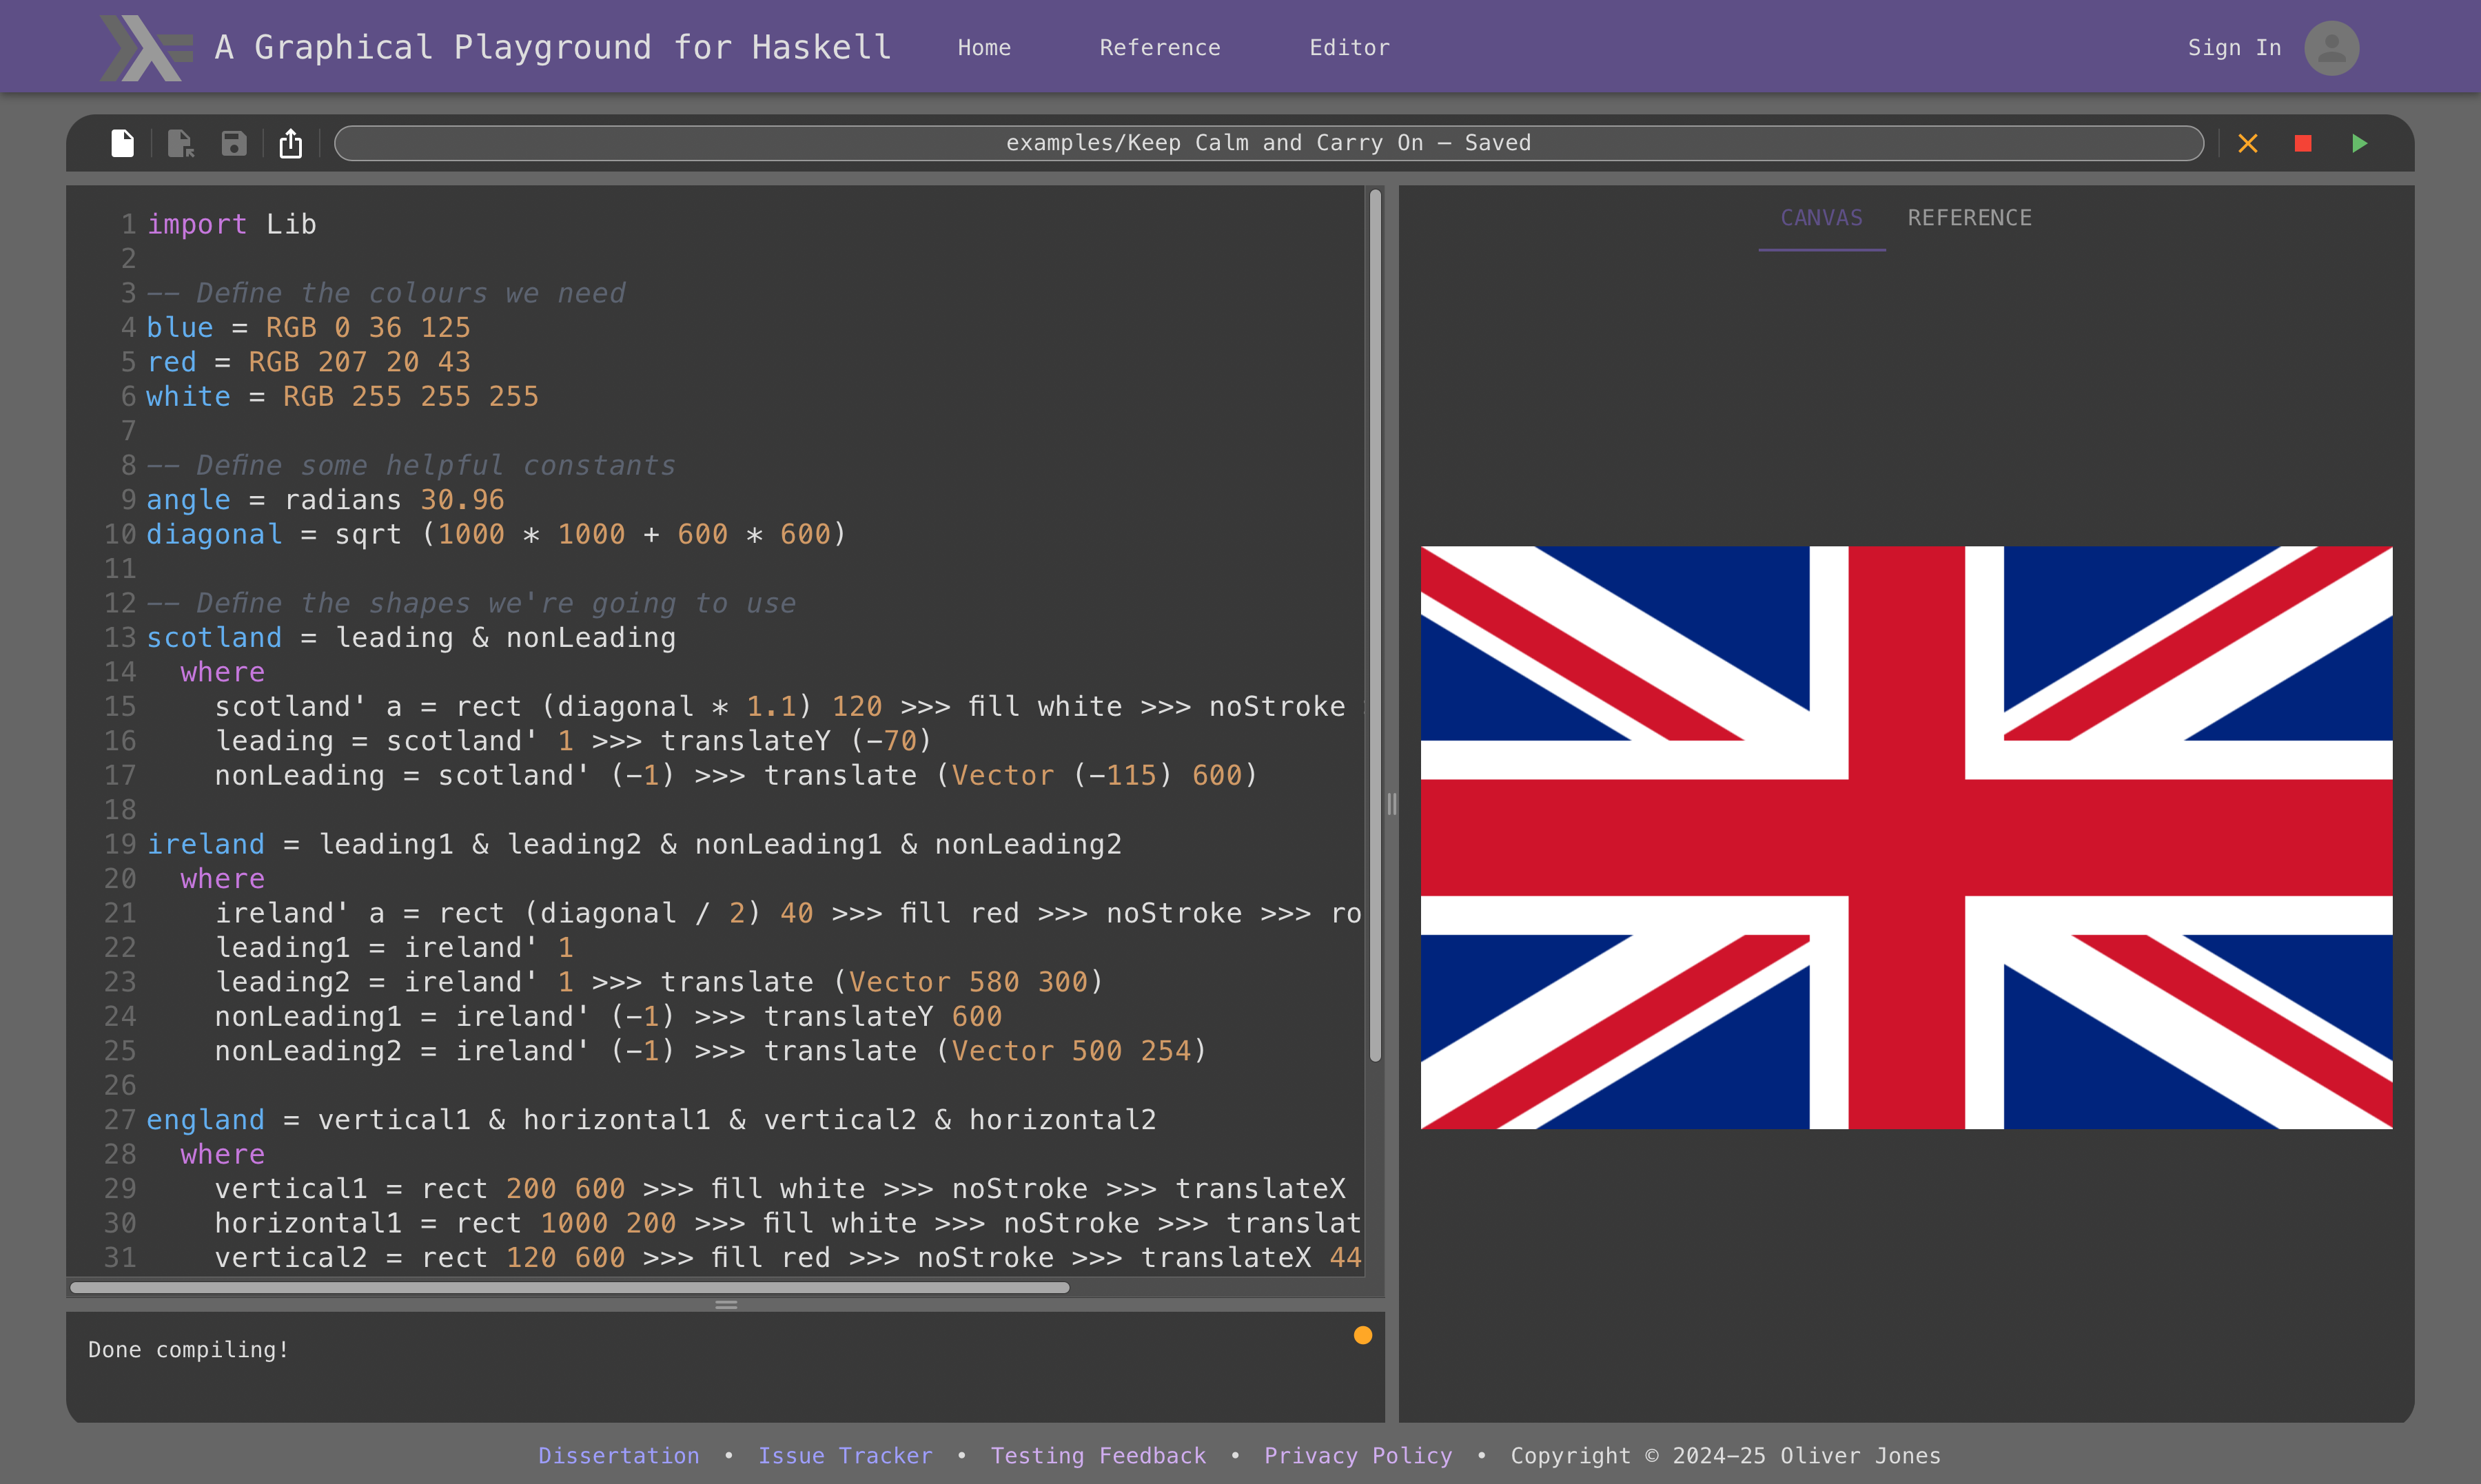
\includegraphics[width=0.75\linewidth]{images/editor.png}
                    \caption{The editor page.
                        At the top is website's header, containing the monochrome Haskell logo to make
                            it visible against the background, the website's name, the navigation links,
                            and a sign-in button.
                        Below are the four editor components outlined above.
                        The toolbar is at the top, the code editor on the left, the graphics display on
                            the right, and the console below the code editor.
                    }
                    \label{fig:editor}
            \end{figure}

            \subsubsection{The Code Editor}
                There are a wide variety of elements built-in to HTML.
                One of these is the \texttt{<textarea>} element, which creates a multi-line
                    text input.
                This can be used to create a simple code editor.
                Unfortunately, you cannot change the colour of individual parts of the text in
                    a \texttt{<textarea>} element, so it is not suitable for syntax highlighting.

                This posed a challenge, as a good code editor should provide syntax
                    highlighting to help users identify parts of their code.
                The solution was to layer another element, in this case the \texttt{<pre>}
                    element, behind the \texttt{<textarea>} element, then setting the background
                    and text colours of the \texttt{<textarea>} to \texttt{transparent}.
                The \texttt{<pre>} element preserves whitespace and line breaks, making it
                    ideal for displaying code.

                An event listener was added to the \texttt{<textarea>} element, which listens
                    for changes to the text.
                The content of the \texttt{<pre>} element was then updated with the
                    syntax-highlighted version of the code whenever the user types.
                The \texttt{highlight.js} library was used to provide syntax highlighting.
                This supports multiple languages, and colour themes.
                It wraps keywords in \texttt{<span>} elements with a class corresponding to the
                    type of keyword, which can then be styled using CSS.

                A second event listener was added the \texttt{<textarea>} element to listen for
                    changes to the scroll position, and update the scroll position of the
                    \texttt{<pre>} element accordingly.
                By setting the \texttt{font-size}, \texttt{line-height} and
                    \texttt{letter-spacing} CSS properties of both the \texttt{<textarea>} and
                    \texttt{<pre>} elements to the same values, the two elements lined up
                    perfectly.
                This created the illusion that the code is typed directly into the
                    \texttt{<pre>} element.

                Another useful feature of a code editor is automatic line numbering, which can
                    help users keep track of where they are in their code.
                To achieve this, each line was split into a separate \texttt{<code>} element.
                The line number was then rendered using the \texttt{::before} pseudo-element in
                    CSS, which can insert extra content before an element.
                CSS also provides a built-in \texttt{counter()} function, which can be used to
                    automatically number the lines of code.

            \subsubsection{The Console}
                This was the simplest component to implement as it is just displays the output
                    of the user's program as it runs.
                A simple React component which receives a string as an input and renders it as
                    a block of text was all that was needed initially.
                Later, this component was expanded to include a status indicator, which
                    displays whether the program is currently running, has finished, or raised an
                    error.
                Originally, this was indicated with extra text in the console, but this proved
                    to be confusing for users.

            \subsubsection{The Graphics Display}
                The original plan for this component was quite simple, just a canvas element,
                    with a function to parse the JSON output of the user's program and draw the
                    graphics on the canvas.
                However, this was more complex than anticipated.
                Due to the nature of React, when a component's state updates, the component and
                    its children are re-rendered.
                With the user's code stored in the state of the editor component, changes to
                    the code caused the editor component to re-render, triggering all of its
                    children to re-render as well.
                This posed an issue for the graphics component, as every re-render would, at
                    best, cause a small flicker as the rendered image is re-rendered, and at worst,
                    cause an animation to restart.
                Fortunately, React provides a solution to this problem.
                The graphics component was memoised using the \texttt{React.memo} function,
                    meaning that it would only re-render when its props change, rather than when
                    its parent component re-renders.

                With this solution, it was straightforward to wait for the user's program to
                    finish running, then parse the output and draw the graphics on the canvas.
                However, this meant that the user had to wait for the program to finish running
                    before they could see any graphics.
                By implementing an intermediate controller component, the graphics could be
                    drawn as the program runs, allowing the user to see the graphics being drawn in
                    real-time.
                This intermediate component was also memoised, so it only re-rendered as more
                    data was received from the server.
                It was then responsible for parsing the JSON data, and passing it to the
                    graphics component to be drawn on the canvas at the correct time, based on the
                    frame rate of the animation.

            \subsubsection{The Toolbar}
                \begin{figure}[H]
                    \centering
                    
\includegraphics[width=\linewidth]{images/toolbar.png}
                        \caption{The toolbar component.}
                        \label{fig:toolbar}
                \end{figure}

                On the left are four buttons: new, save, open and share.
                As the names suggest, these buttons allow users to create a new program,
                    replacing the content of the code editor with some boilerplate code, save their
                    current program, open a saved program, and share their program.
                Saving and opening programs are only available to users who are logged in.
                Sharing programs is available to all users.
                Sharing gives the user the option of copying their program to the clipboard,
                    generating and copying a URL which links directly to the program, copying the
                    image output of the program to the clipboard, or downloading the image output
                    of the program.
                The name of the program is displayed in the centre of the toolbar, along with
                    the name of the user who wrote it.
                To the right are three buttons: clear, run and stop.
                The clear button clears the console and graphics display, the run button runs
                    the user's program, and the stop button stops the program if it is currently
                    running.

        \subsection{Making the Components Resizable}
            Making the components resizable was relatively straightforward.
            A custom \texttt{SplitView} component was created, which takes two child
                components, and creates a draggable border between them.
            Using this component twice created a three-way split view.
            A simplified version of the layout is shown in Listing~\ref{lst:editorLayout}.

            \begin{lstlisting}[caption={A simplified version of the editor page layout.}, 
                label={lst:editorLayout}]
<SplitView>
    <SplitView vertical>
        <CodeEditor />
        <Console />
    </SplitView>
    <GraphicsController />
</SplitView>\end{lstlisting}

            While React allows any HTML element to be marked as \texttt{draggable}, this
                causes the element to be movable in both the x and y directions, which can
                cause strangle visual artefacts when dragging the border.
            To prevent this, a React state variable was used to store whether the user is
                currently dragging the border.
            When the user clicks on the border, this variable was set to \texttt{true}, and
                when the user releases the mouse button, it is set back to \texttt{false}.
            An event listener was then added to check for mouse movements.
            If the dragging variable is \texttt{true}, we would update the sizes of the two
                child components based on the mouse position.
            This produced two resizable components without any visual artefacts.

    \section{Making a Reference Page}
        The reference page was considerably simpler to implement than the editor page.
        It is simply a long page of text, with a table of contents at the top, linking
            to the various sections of the page.
        The page was divided into sections, with alternating coloured backgrounds to
            make it easier to read.
        Each section detailed a different aspect of the graphics library:
        \begin{itemize}
            \item ``Haskell'', with a brief explanation of Haskell's \texttt{Prelude} module,
                  a link to its full documentation, and an explanation of Haskell's type
                  signature syntax.
            \item ``Canvas'', to explain the concept of the canvas, and how to create it.
            \item ``Images and Animations'', to explain how to draw images and animations on the
                  canvas and modify the frame rate and background colour.
            \item ``Vectors'', to explain how to create and manipulate vectors.
            \item ``Shapes'', to explain how to create the various shapes available in the
                  graphics library, with pictures of each shape.
            \item ``Transformations'', to explain how to manipulate these shapes, with pictures
                  of each transformation.
            \item ``Colors'', to explain how to create colours using the various colour spaces
                  available in the graphics library.
            \item ``Other'', to explain how to use the other functions available in the graphics
                  library.
        \end{itemize}

        Throughout the page are a series of examples, demonstrating how to use the
            functions available in the graphics library.
        These are written in both inline and block code, which are styled accordingly
            to make them clear.

        \begin{figure}[H]
            \centering
            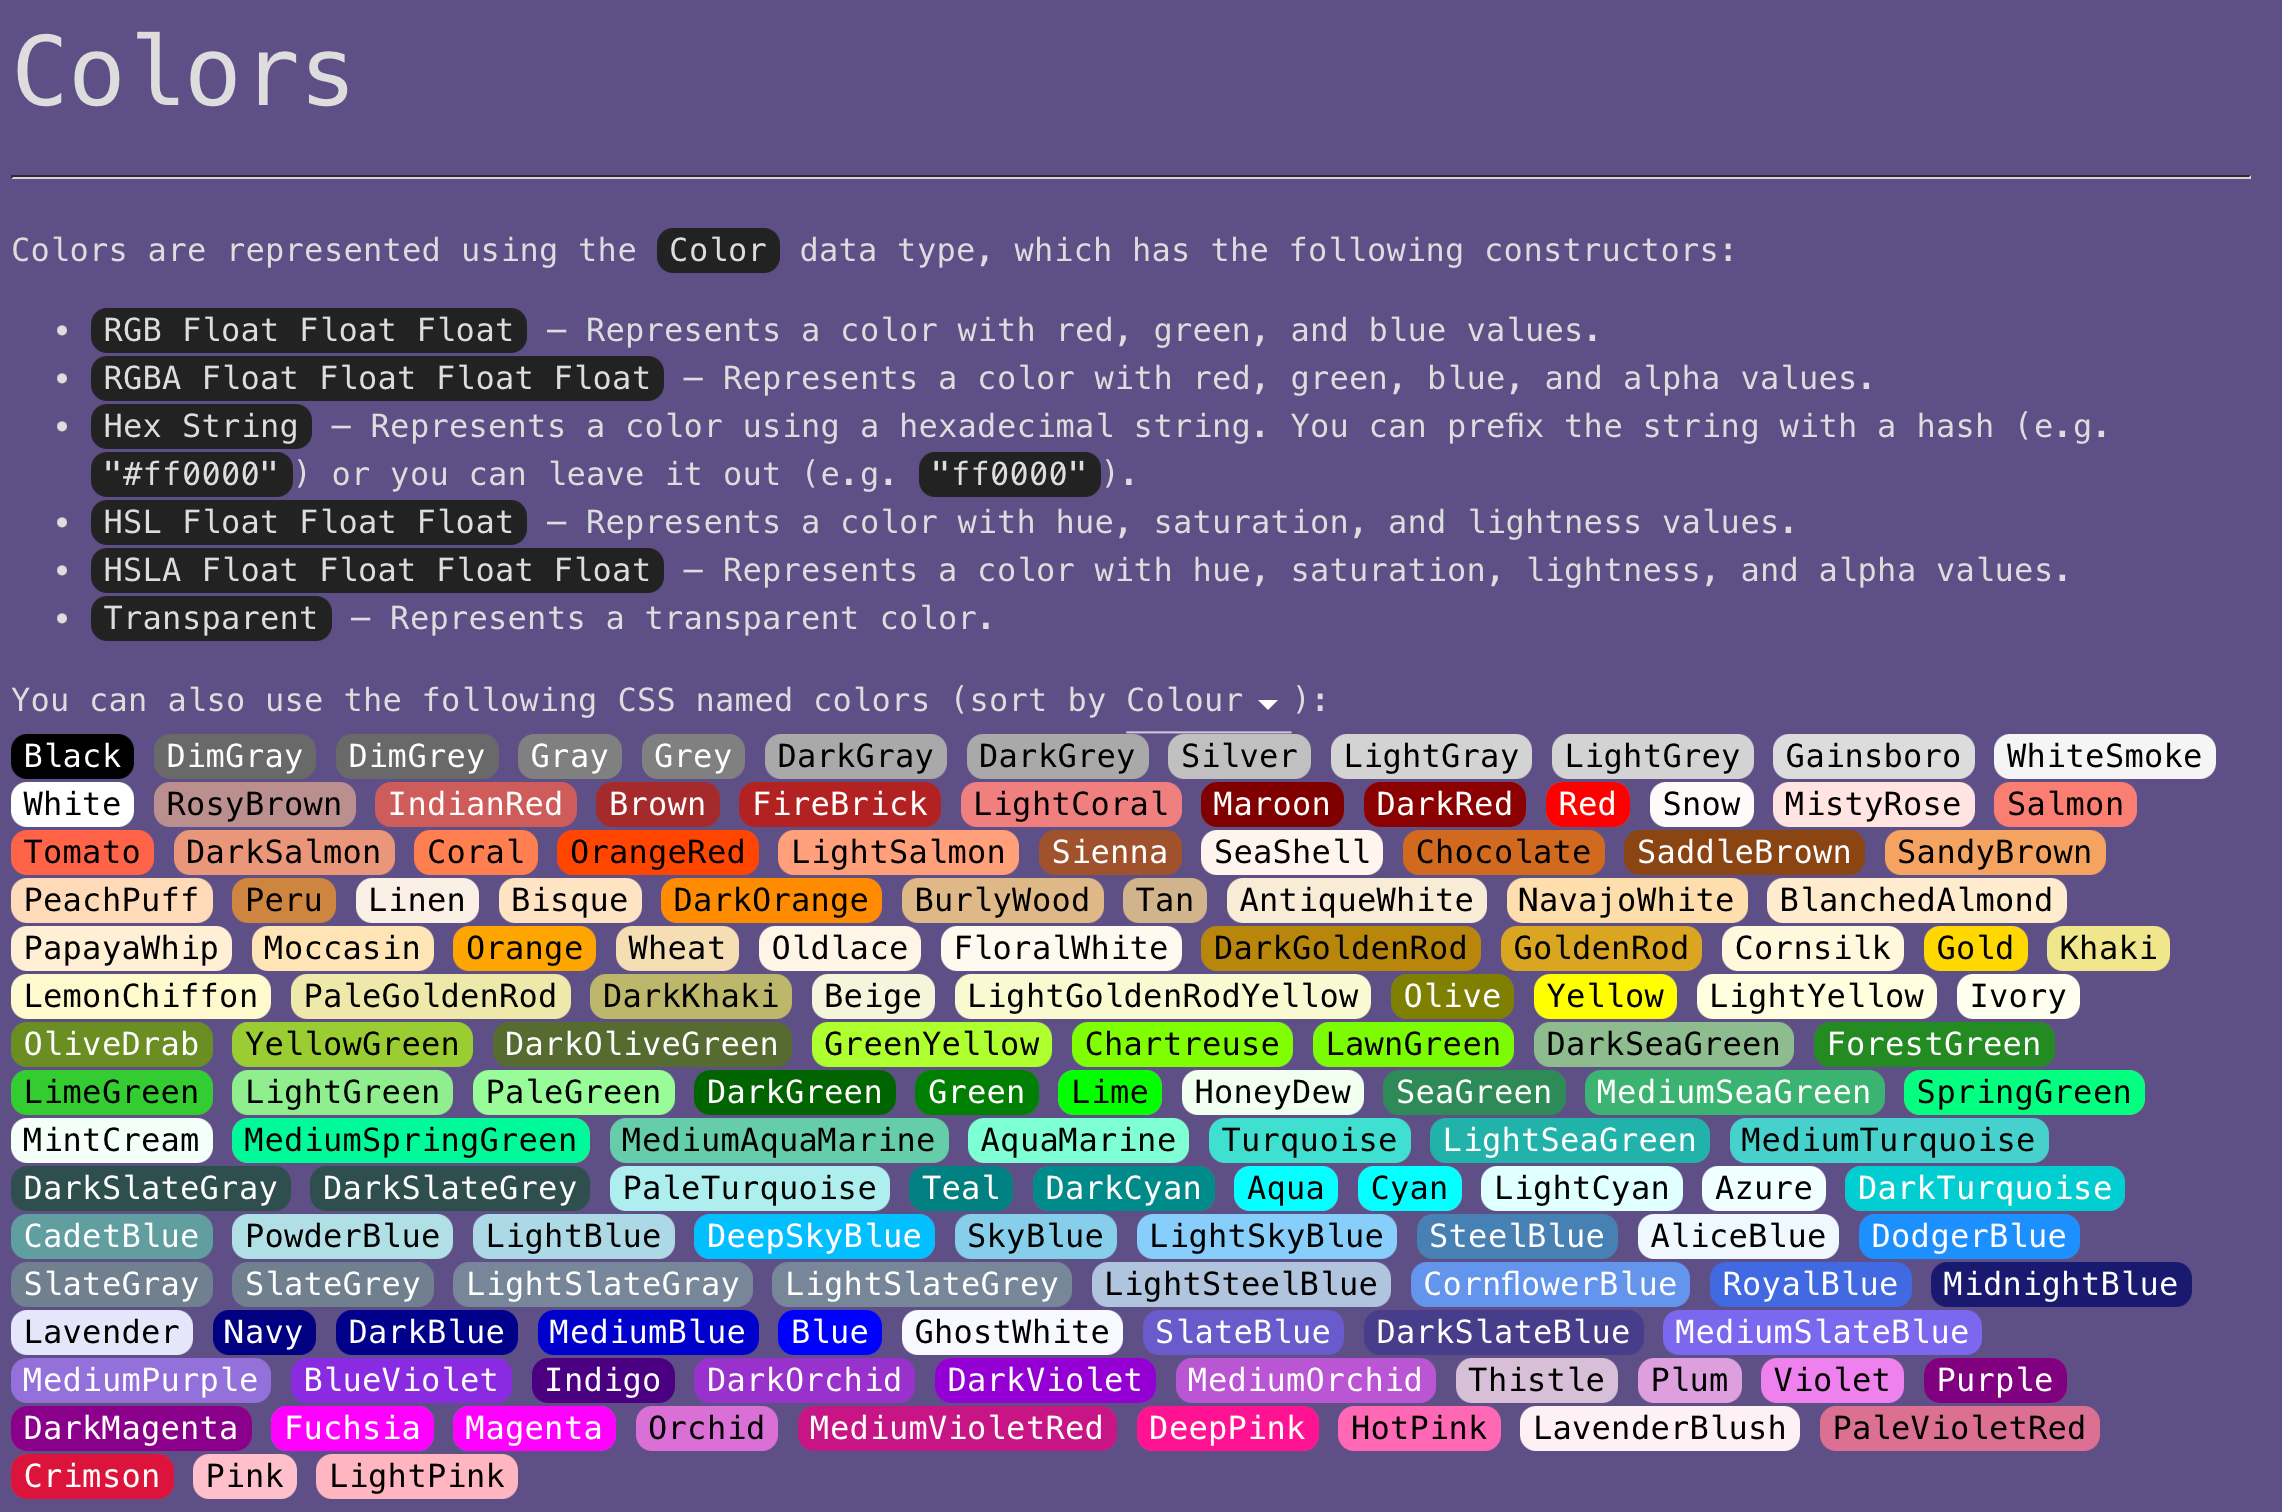
\includegraphics[width=0.45\linewidth]{images/colours.png}
            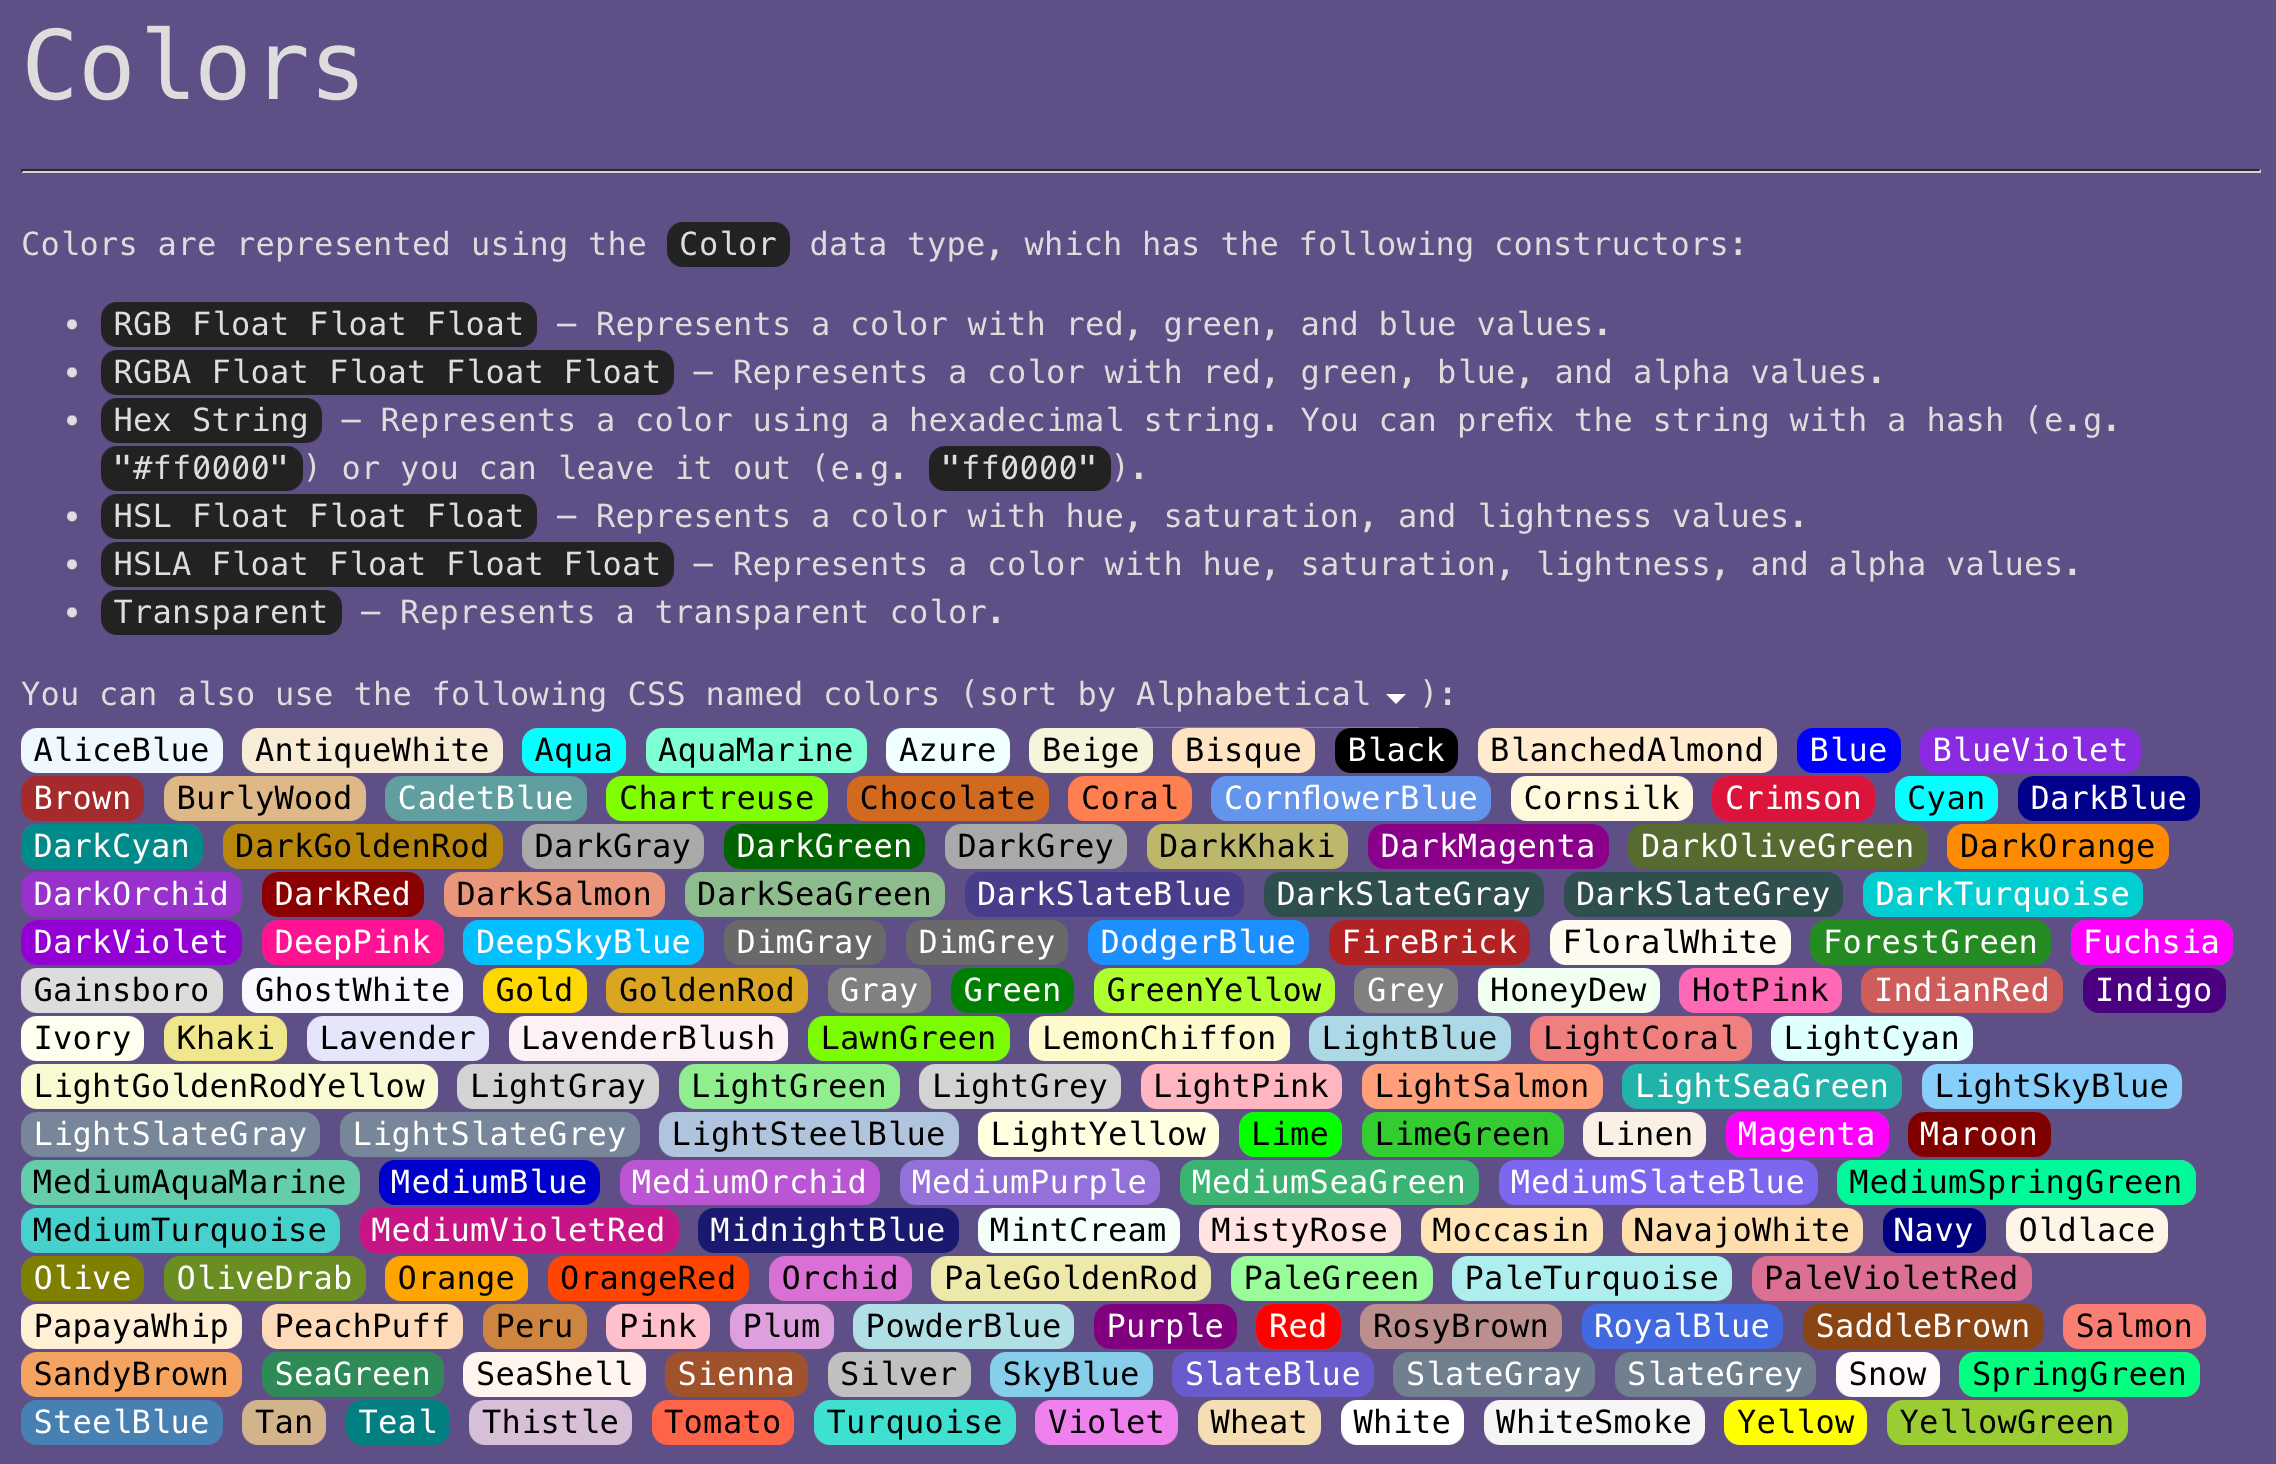
\includegraphics[width=0.45\linewidth]{images/coloursAlphabetical.png}
                \caption{The ``Colors'' section of the reference page.
                    On the left, the colours are sorted by hue, saturation, and lightness.
                    On the right, the colours are sorted alphabetically.
                }
                \label{fig:colours}
        \end{figure}

        The ``Color'' section also includes a list of all the named colours available
            in the graphics library (see Figure~\ref{fig:colours}).
        Each colour is displayed as its name, highlighted in that colour.
        Hovering over these displays a tooltip with the hexadecimal, RGB and HSL values
            of the colour.
        The list can be sorted either by colour, a combination of hue, then saturation,
            then lightness, or alphabetically by name, to accommodate users who are
            colour-blind.

    \section{Creating a User Account System}
        User accounts are nothing new to the internet.
        They are used for storing user data, and to provide a more personalised
            experience for the user.
        For this website, user accounts were used to store the user's saved programs.

        Next.js provides built-in support for middleware, which can be used to direct
            users to the correct page based on their authentication status.
        Users who are not logged in, who try to access the account page, are redirected
            to the login page.
        Users who are logged in, who try to access the login page, are redirected to
            the account page.
        This ensures that users are always directed to the correct page, based on their
            authentication status.

        The user account system is relatively simple.
        Users can create an account by providing an email address and password.
        The password is hashed using the \texttt{bcrypt} library, and the email address
            is stored in plain text.
        When a user logs in, the server checks the email address and password against
            the database, and if they match, the user is logged in.
        A unique identifier is generated for the user, and stored in a cookie, which is
            sent to the client.
        This cookie is used to authenticate the user on subsequent requests, so they do
            not need to log in every time they try to access a protected endpoint.

        The user account system also allows users to save their programs.
        When a user saves a program, it is stored in the database, along with the
            user's unique identifier.
        When a user logs in, the server retrieves all the programs associated with that
            user's unique identifier, and displays them on the account page.

    \section{Landing on the Homepage}
        The homepage is the first page users see when they visit the website.
        It is designed to be engaging and informative, showcasing the capabilities of
            the graphics library, and encouraging users to try it out.

        The top of the homepage features a large banner, indicating the name of the
            website.
        Below is a brief welcome message, encouraging users to try out the graphics
            library.
        Below this is a series of examples, showcasing the capabilities of the graphics
            library — both static images and animations.
        Finally, at the bottom of the page is a help section, directing users to the
            reference page for more information about the graphics library, and to the
            issue tracker if they encounter any problems.

        \begin{figure}[H]
            \centering
            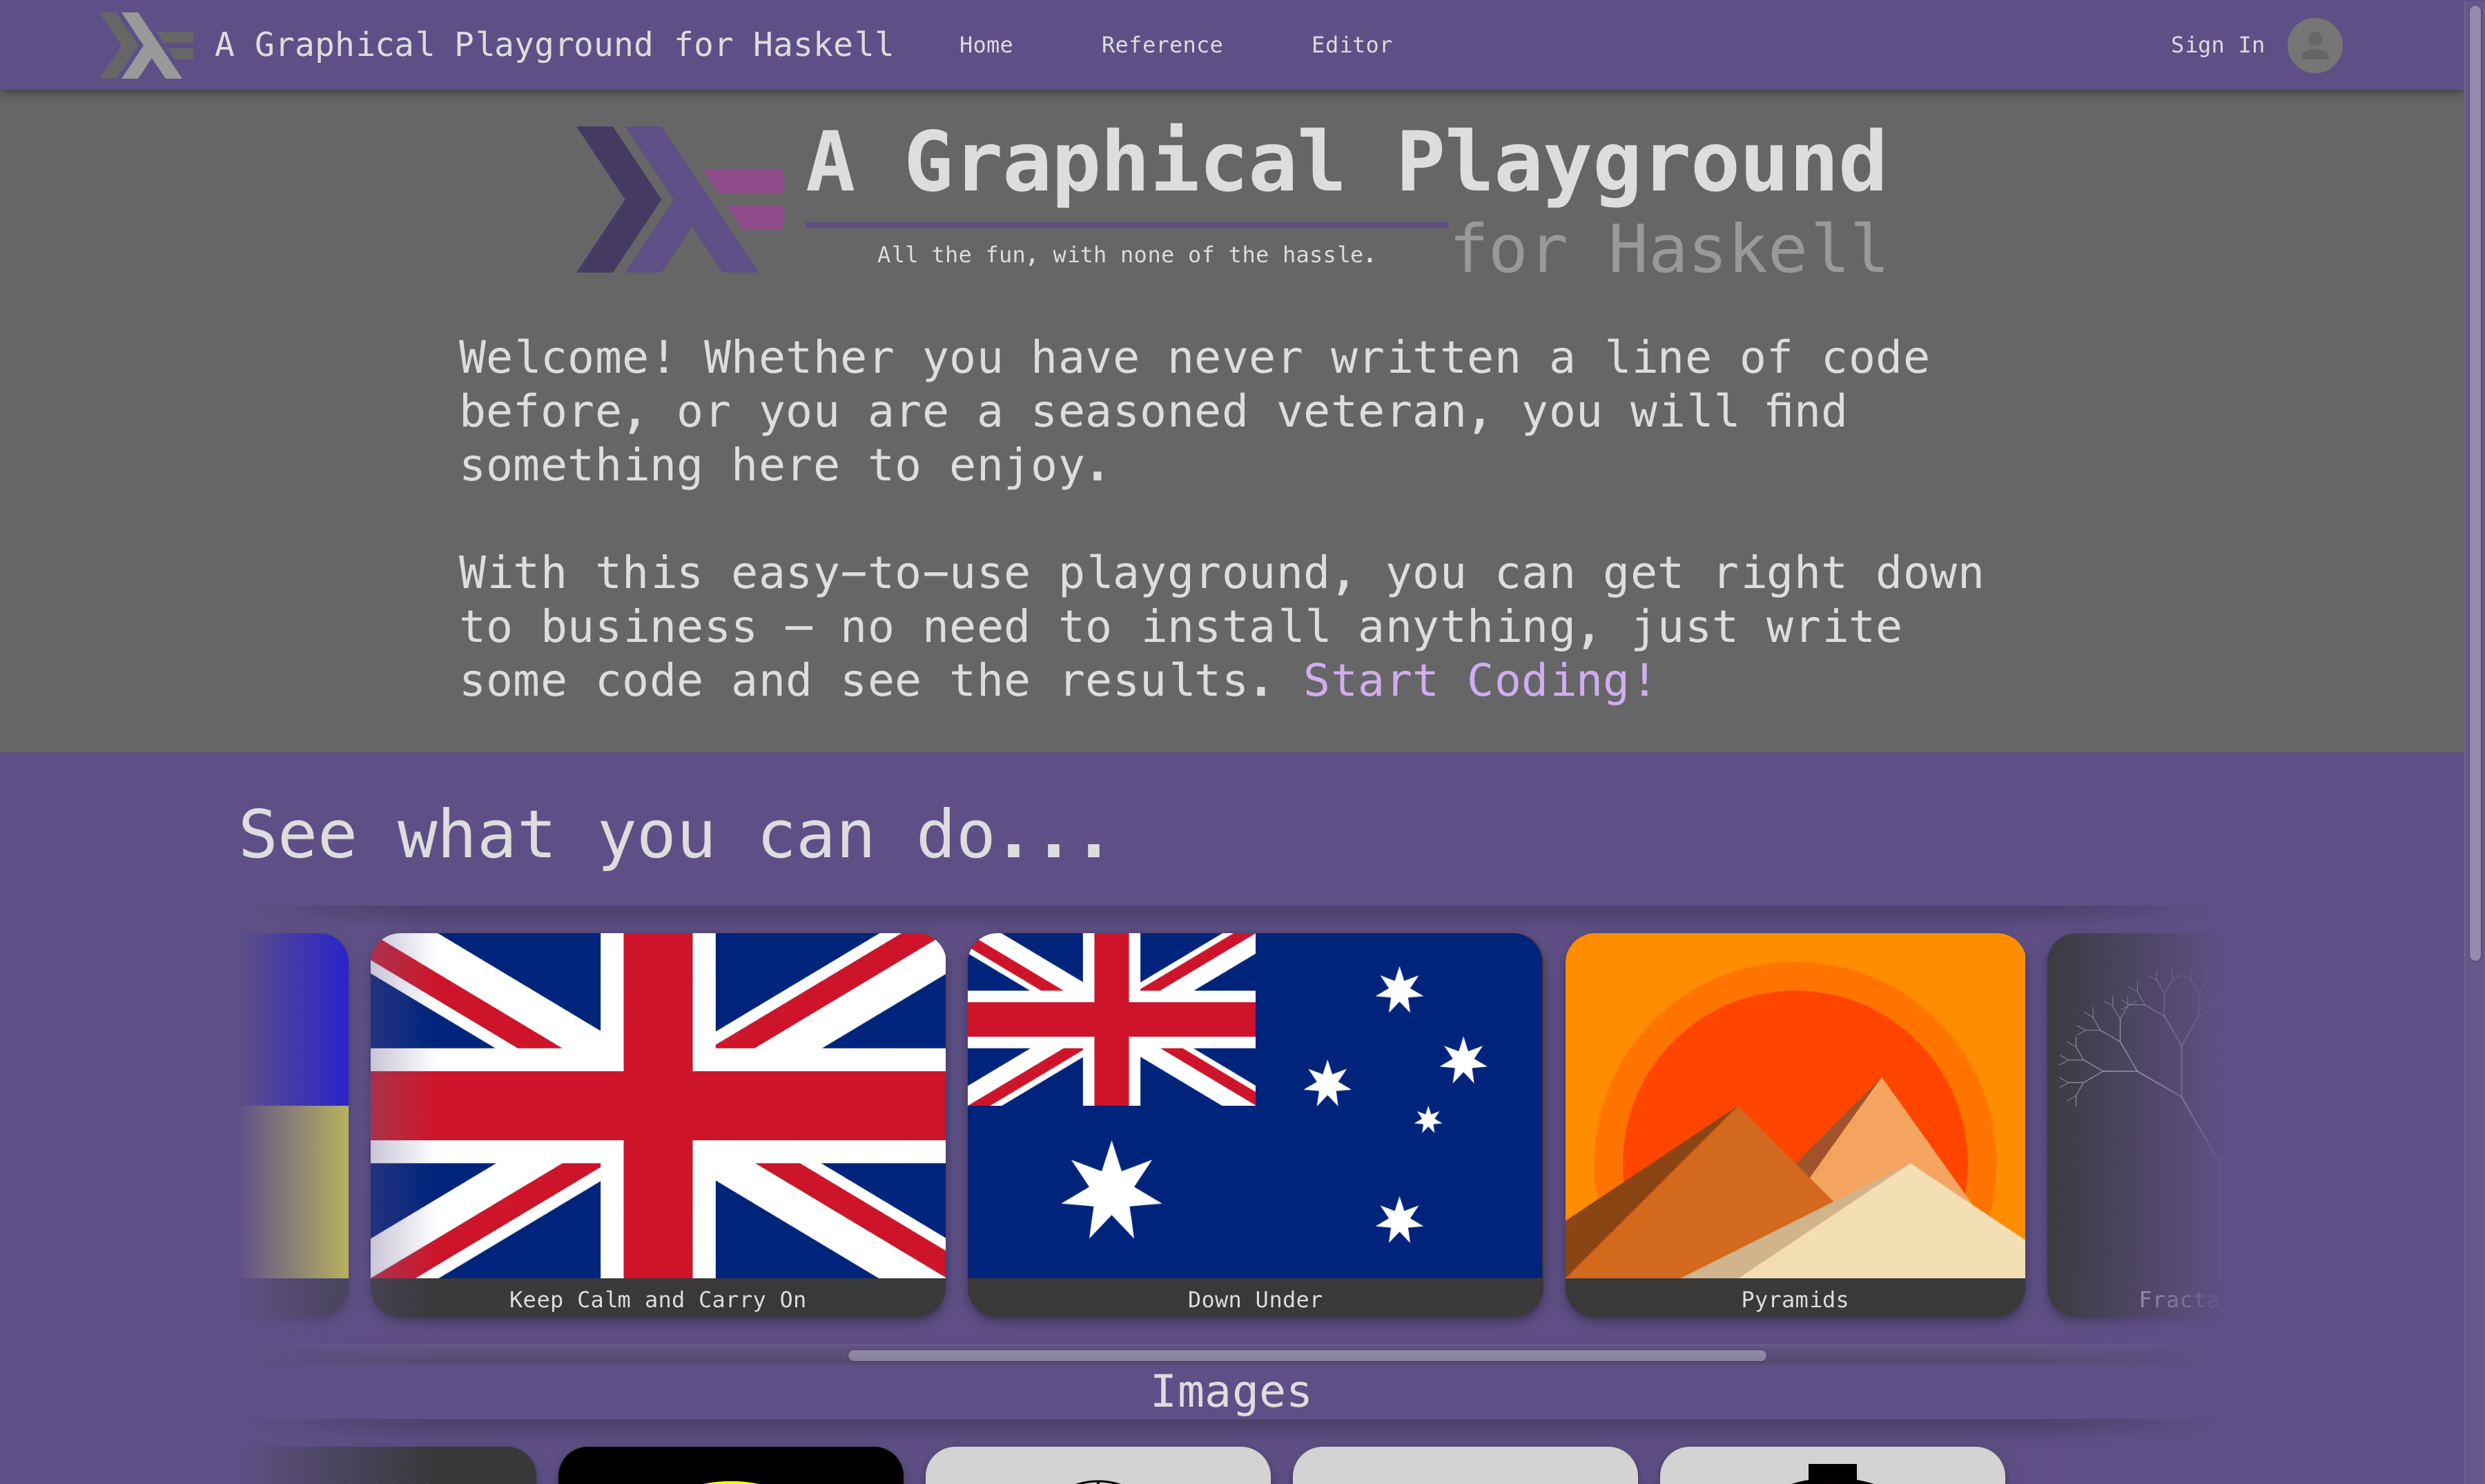
\includegraphics[width=0.75\linewidth]{images/homepage.png}
                \caption{The homepage.}
                \label{fig:homepage}
        \end{figure}

    \section{Quality-of-Life and Legal Requirements}
        There were a few features that were added to the website to make it more
            user-friendly, and to comply with legal requirements.
        These included:
        \begin{itemize}
            \item A notification banner which appears at the bottom corner of the screen
                  whenever a user carries out certain actions such as saving a program, copying
                  their program or URL via the share, etc.
                  The banner automatically fades after a few seconds, but does not disappear
                      entirely until the user dismisses it.
            \item A notification informing the user that the website uses cookies, as is legally
                  required by GDPR regulations.
                  This makes use of the same notification banner as the other notifications, and
                      includes a link to the privacy policy.
            \item The footer includes links to this dissertation, the GitHub issue tracker,
                  the user testing and feedback form, and the privacy policy.
                  The privacy policy is a legal requirement, and outlines how the website
                      collects, stores and uses user data.
                  It also includes a copyright notice.
                  While this is not strictly necessary, as UK copyright law protects the author's
                      rights to their work, regardless of whether they include a copyright notice, it
                      is a good practice to include one, as many users may not be aware of this.
            \item A saved state indicator appears in the menu bar, informing a user of whether
                  they have an open program, and if it is saved.
                  Hovering over this indicator displays a tooltip with the name of the program.
            \item Confirmation menus appear when a user tries to open a program while they
                  have an unsaved program open, preventing them from losing their work.
                  The same is true when a user tries to delete one of their saved programs.
        \end{itemize}

\end{document}
